\documentclass[class=beamer, crop=false]{standalone}
\usepackage{tikz}
\usepackage{subcaption}
\usetikzlibrary{calc}

\begin{document}

% \begin{figure}
%   \centering
\begin{minipage}{0.24\textwidth}
    \centering
  % ─── Panel 1 ─────────────────────────────
  \begin{minipage}[t]{0.24\textwidth}
    \centering
    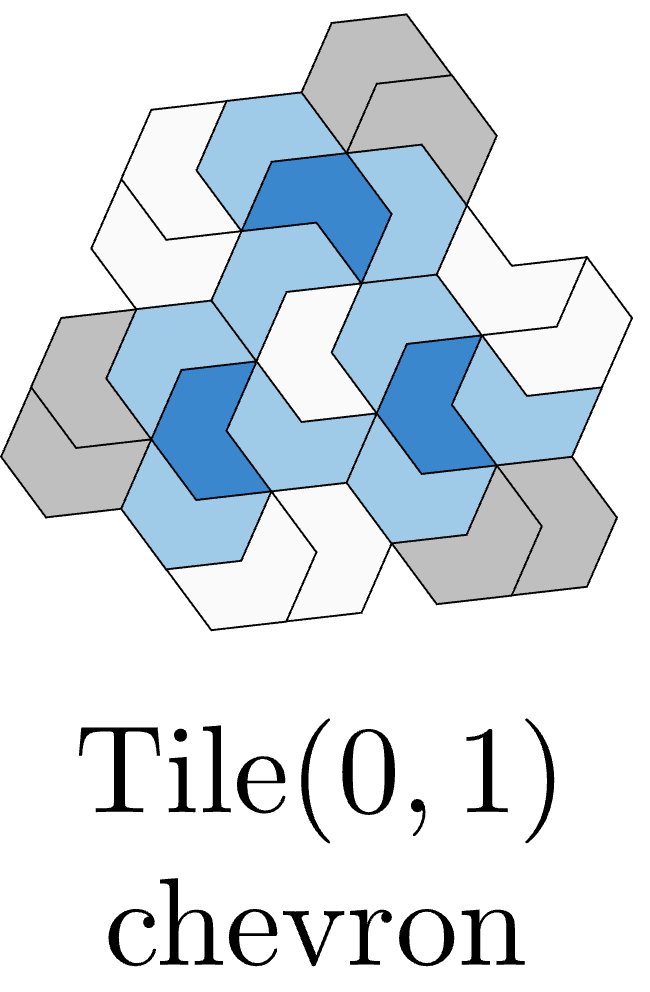
\includegraphics[width=\linewidth]{images/polykite-family/chevron(0,1).png}
    % \caption*{Chevron $(0,1)$}   % <-- optional sub-caption
  \end{minipage}\hfill
  % ─── Panel 2 ─────────────────────────────
  \begin{minipage}[t]{0.24\textwidth}
    \centering
    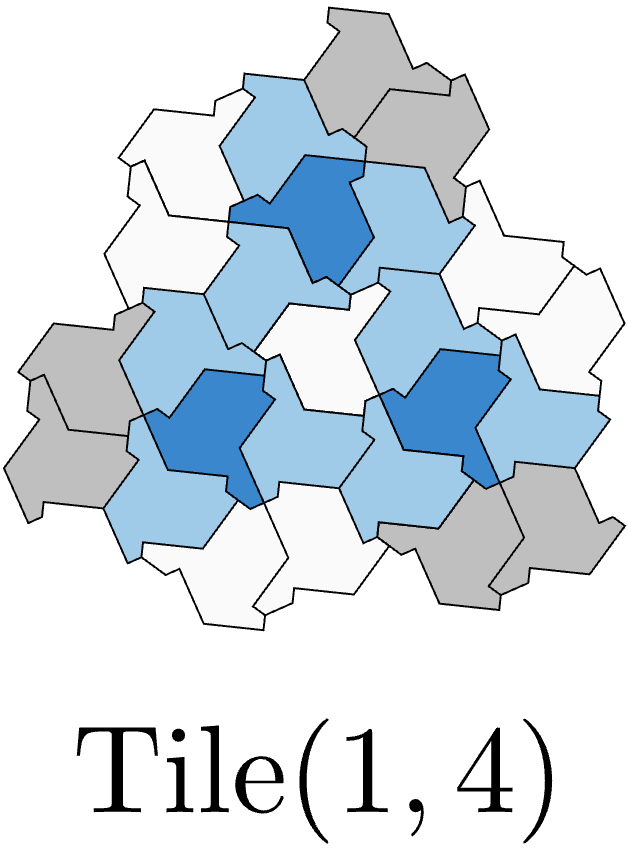
\includegraphics[width=\linewidth]{images/polykite-family/tile(1,4).png}
    % \caption*{Tile $(1,4)$}
  \end{minipage}\hfill
  % ─── Panel 3 ─────────────────────────────
  \begin{minipage}[t]{0.24\textwidth}
    \centering
    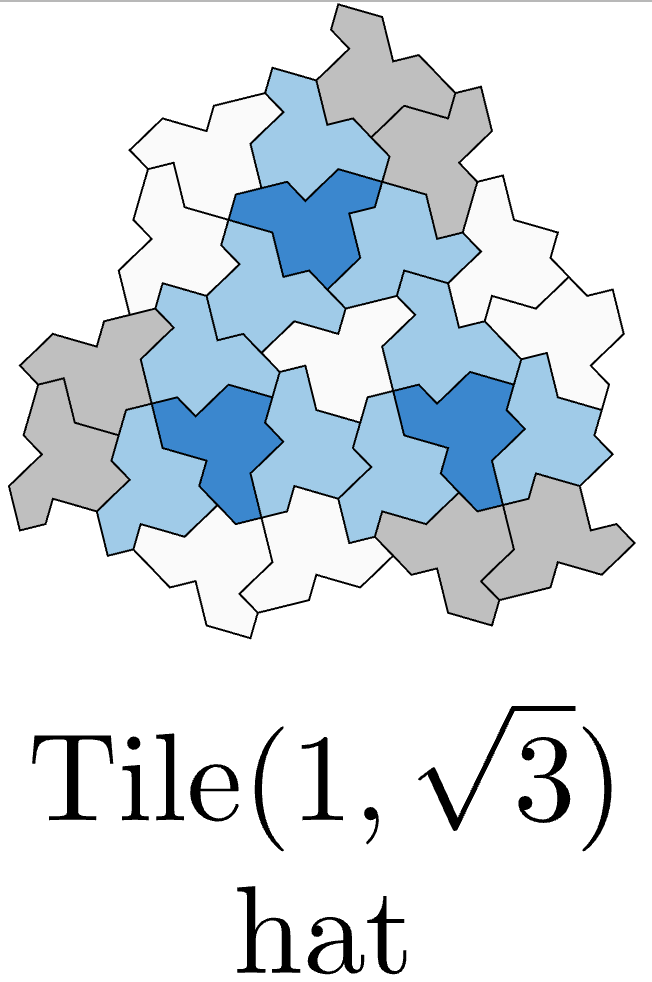
\includegraphics[width=\linewidth]{images/polykite-family/hat(1,sqrt(3)).png}
    % \caption*{Hat $(1,\sqrt3)$}
  \end{minipage}\hfill
  % ─── Panel 4 ─────────────────────────────
  \begin{minipage}[t]{0.24\textwidth}
    \centering
    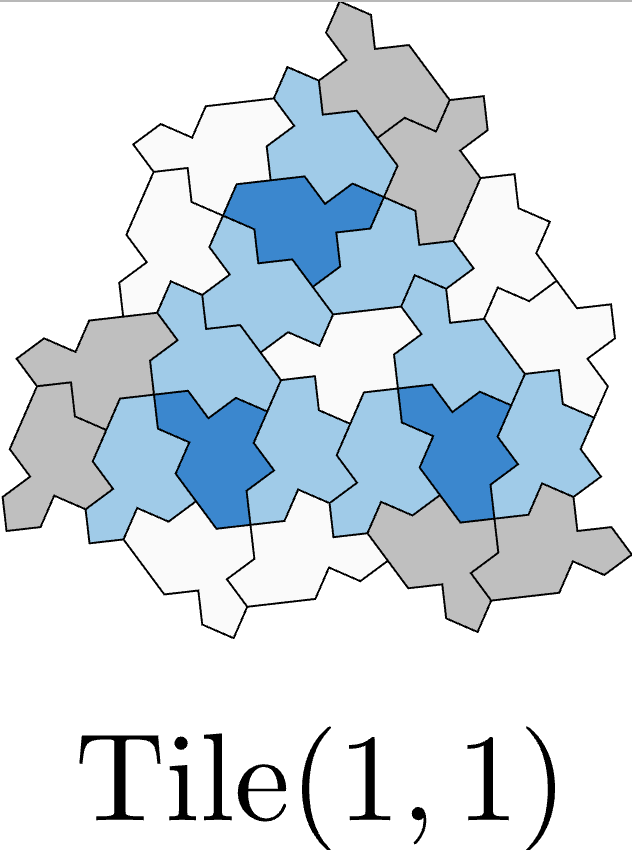
\includegraphics[width=\linewidth]{images/polykite-family/tile(1,1).png}
    % \caption*{Tile $(1,1)$}
  \end{minipage}


  \begin{minipage}[t]{0.24\textwidth}
    \centering
    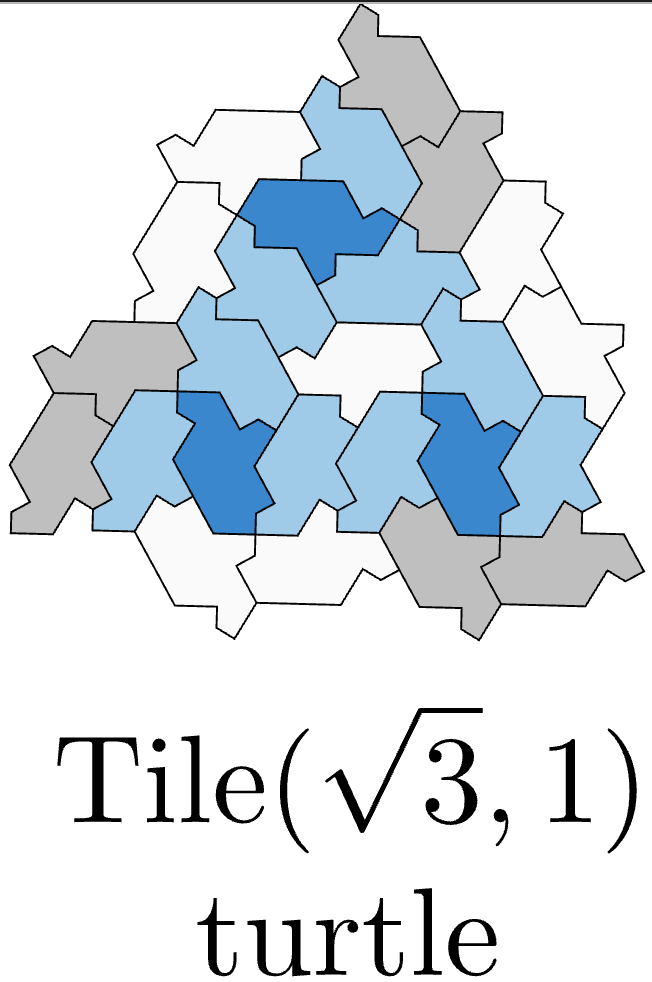
\includegraphics[width=\linewidth]{images/polykite-family/turtle(sqrt(3),1).png}
    % \caption*{Tile $(1,4)$}
  \end{minipage}\hfill
  % ─── Panel 6 ─────────────────────────────
  \begin{minipage}[t]{0.24\textwidth}
    \centering
    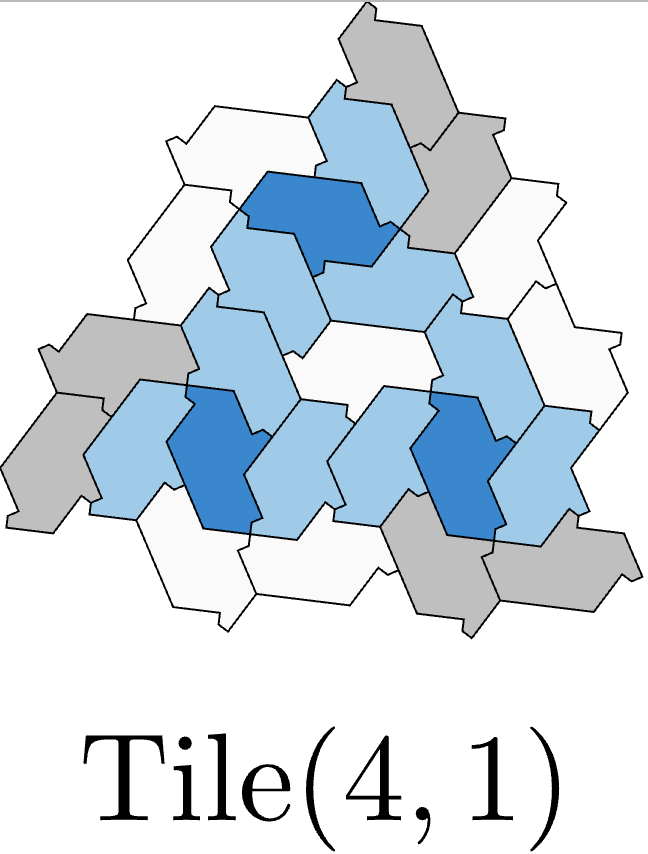
\includegraphics[width=\linewidth]{images/polykite-family/tile(4,1).png}
    % \caption*{Hat $(1,\sqrt3)$}
  \end{minipage}\hfill
  % ─── Panel 7 ─────────────────────────────
  \begin{minipage}[t]{0.24\textwidth}
    \centering
    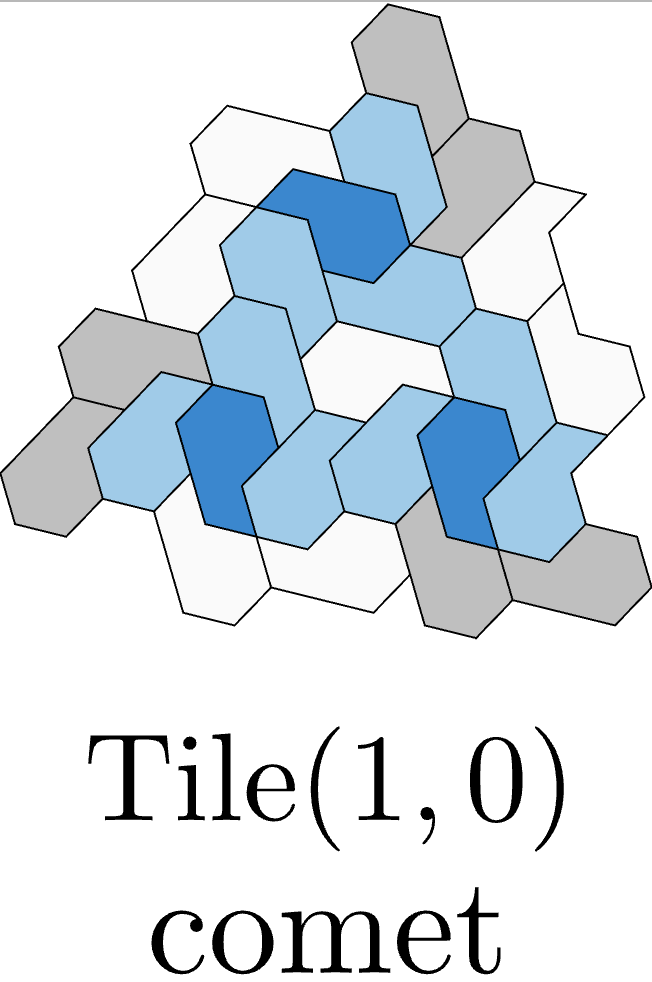
\includegraphics[width=\linewidth]{images/polykite-family/comet(1,0).png}
    % \caption*{Tile $(1,1)$}
  \end{minipage}
\end{minipage}
  % \caption{Tilling of polykite family.}
  % \label{fig:polykite-family}
% \end{figure}

\end{document}